\documentclass[conference]{IEEEtran}
\IEEEoverridecommandlockouts

\usepackage{cite}
\usepackage{amsmath,amssymb}
\usepackage{graphicx}
\usepackage{booktabs}
\usepackage{multirow}
\usepackage{array}
\usepackage{url}
\usepackage{xcolor}
\usepackage{tikz}
\usetikzlibrary{arrows.meta,positioning,fit,calc}

\graphicspath{{figures/}}

\begin{document}

\title{ESP-AGV: On-Device Anomaly Detection and Fault Response for a Line-Following AGV with an ESP32-S3 in the Loop}

% TODO: replace with the team's full names, department, university and emails.
\author{
\IEEEauthorblockN{Author Name 1}
\IEEEauthorblockA{\textit{Department, University}\\
City, Country\\
email@example.com}
\and
\IEEEauthorblockN{Author Name 2}
\IEEEauthorblockA{\textit{Department, University}\\
City, Country\\
email@example.com}
}

\maketitle

\begin{abstract}
We present ESP-AGV, an automated guided vehicle (AGV) whose onboard computer is a
low-cost ESP32-S3 microcontroller connected in the loop to a Webots simulation of
an e-puck robot on a line track. Every 32\,ms the simulator streams three
ground-infrared (IR) readings and two wheel-encoder positions to the ESP32-S3 over
USB serial; the microcontroller runs the line-following controller, odometry-gated
junction and destination logic, four anomaly detectors (motor and IR convolutional
autoencoders, a motor GRU plant model and a stuck-sensor rule), and the fault
response: pulling over to a map-chosen side, stopping and sending a phone
notification over WiFi. Faults are injected only in the simulator, so the ESP
observes them exactly as it would on hardware. On 120 labelled fault runs covering
15 motor, encoder and sensor faults, the deployed detectors flag 94 runs with the
fault's own detector and 110 with either detector, with no alarm before any fault
onset and no alarm on any healthy validation run. All seven motor and encoder fault
types are detected in 8/8 runs with a median delay of 0.10--0.29\,s. Inference uses
Espressif's esp-dsp SIMD library in float32 and costs about 0.81\,ms of each
32\,ms control frame, matching the Python reference within $2.5\times10^{-5}$ with
identical alarm decisions. A multi-objective architecture search driven by
latencies measured on the device found detectors that are 2--3$\times$ faster and
3$\times$ smaller than the hand-designed ones while detecting as many or more
faults. Without retraining any detector, the system also completes all routes,
and stops on every injected fault, on two further tracks not used for training.
\end{abstract}

\begin{IEEEkeywords}
anomaly detection, autoencoder, GRU, embedded machine learning, TinyML,
ESP32-S3, AGV, fault injection, hardware-in-the-loop, Webots
\end{IEEEkeywords}

%=====================================================================
\section{Introduction}
%=====================================================================
Automated guided vehicles move material along fixed paths in factories and
warehouses. A worn motor, a slipping wheel or a dirty floor sensor degrades such
a vehicle gradually; detecting the degradation on the vehicle itself, before it
leaves its path, avoids both downtime and collisions. Running the detector on the
vehicle's own microcontroller keeps the response independent of network links
and adds no hardware.

This project builds such a system end to end on an ESP32-S3
microcontroller~\cite{esp32s3} with the physical environment simulated in
Webots~\cite{webots}. The microcontroller is not a model of the robot's
computer: it \emph{is} the computer, receiving sensor data and returning wheel
commands every 32\,ms. Faults are injected in the simulator, so the
microcontroller must detect them from its inputs alone.

The contributions are:
\begin{itemize}
\item a hardware-in-the-loop AGV in which an ESP32-S3 performs line following,
  graph-route execution with odometry-gated junctions, and round trips;
\item four complementary anomaly detectors trained only on healthy data and
  deployed on the ESP32-S3 with esp-dsp~\cite{espdsp}, matching their Python
  reference frame by frame;
\item an autonomous fault response (pull-over side chosen from the map, stop,
  phone notification);
\item a fault-injection and evaluation pipeline with 9 fault mechanisms, run-level
  data splits, severity sweeps and live tests, and a hardware-aware architecture
  search using latencies measured on the device.
\end{itemize}

%=====================================================================
\section{System Design and Architecture}
%=====================================================================

\subsection{Overview}
Fig.~\ref{fig:architecture} shows the three layers. Webots simulates an e-puck
robot with three downward-facing ground sensors on a 1\,m\,$\times$\,1\,m
arena whose floor texture is the track. A Python controller in Webots acts as the
bridge: it plans the route, sends it once per leg, and then exchanges one sensor
frame and one motor frame with the ESP32-S3 per simulation step. The ESP32-S3
(N16R8, ESP-IDF 6.0.1) computes everything else.

\begin{figure}[t]
\centering
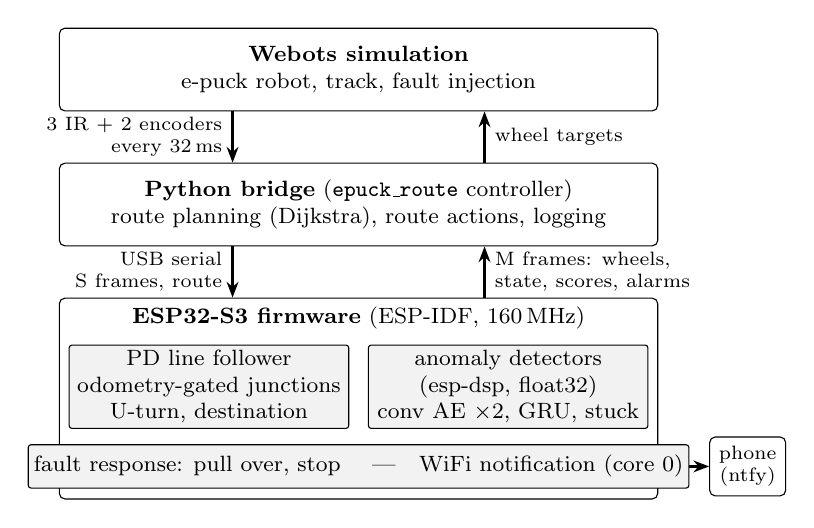
\begin{tikzpicture}[
  font=\footnotesize,
  box/.style={draw, rounded corners=2pt, align=center, minimum width=7.6cm, inner sep=3pt},
  sub/.style={draw, rounded corners=1pt, align=center, fill=gray!10, minimum height=0.55cm, inner sep=2pt},
  arr/.style={-{Stealth[length=2mm]}, thick}]
\node[box, minimum height=1.05cm] (webots) {\textbf{Webots simulation}\\e-puck robot, track, fault injection};
\node[box, below=0.65cm of webots, minimum height=1.05cm] (bridge) {\textbf{Python bridge} (\texttt{epuck\_route} controller)\\route planning (Dijkstra), route actions, logging};
\node[box, below=0.65cm of bridge, minimum height=2.55cm] (esp) {};
\node[anchor=north] at (esp.north) {\textbf{ESP32-S3 firmware} (ESP-IDF, 160\,MHz)};
\node[sub, minimum width=3.55cm] (ctrl) at ($(esp.center)+(-1.9,0.15)$) {PD line follower\\odometry-gated junctions\\U-turn, destination};
\node[sub, minimum width=3.55cm] (det) at ($(esp.center)+(1.9,0.15)$) {anomaly detectors\\(esp-dsp, float32)\\conv AE $\times$2, GRU, stuck};
\node[sub, minimum width=7.3cm] (resp) at ($(esp.south)+(0,0.42)$) {fault response: pull over, stop \quad|\quad WiFi notification (core 0)};
\node[draw, rounded corners=2pt, right=0.25cm of resp.east, anchor=west, align=center, font=\scriptsize] (phone) {phone\\(ntfy)};
\draw[arr] ($(webots.south)+(-1.6,0)$) -- node[left, align=right, font=\scriptsize] {3 IR + 2 encoders\\every 32\,ms} ($(bridge.north)+(-1.6,0)$);
\draw[arr] ($(bridge.north)+(1.6,0)$) -- node[right, align=left, font=\scriptsize] {wheel targets} ($(webots.south)+(1.6,0)$);
\draw[arr] ($(bridge.south)+(-1.6,0)$) -- node[left, align=right, font=\scriptsize] {USB serial\\S frames, route} ($(esp.north)+(-1.6,0)$);
\draw[arr] ($(esp.north)+(1.6,0)$) -- node[right, align=left, font=\scriptsize] {M frames: wheels,\\state, scores, alarms} ($(bridge.south)+(1.6,0)$);
\draw[arr] (resp.east) -- (phone.west);
\end{tikzpicture}
\caption{System architecture. The ESP32-S3 is the robot's computer; Webots
provides the environment and the faults.}
\label{fig:architecture}
\end{figure}

\subsection{Map and route planning}
The track image (2400\,$\times$\,1800\,px) is converted to a named graph of four
junctions and six edges, including two parallel pairs, with a calibrated
pixel-to-world transform. Routes are planned with Dijkstra's
algorithm and converted to a sequence of junction actions
(left, straight, right, bear, corner, destination), each tagged with the
expected odometry distance. Four two-edge routes (A--D) are used throughout;
a round trip returns to the start after a 1\,s unload, beginning with a U-turn.

\subsection{Control design}
The ESP32-S3 steers from the three ground sensors with a PD controller
($K_p=1.2$, $K_d=0.015$, derivative low-pass filtered and limited). Junctions
cannot be identified from the sensor pattern alone: the line is about as wide as
the sensor array, so all three sensors read dark on ordinary wide stretches.
The firmware therefore accepts a junction pattern only within $\pm0.10$\,m of the
odometry distance sent with the route, using per-edge odometry scales
(0.973 on long edges, 0.836 on the curved loop) fitted to 237 recorded legs.

\subsection{Anomaly detection design}
Detection runs on the ESP for every frame, in parallel with control:
\begin{itemize}
\item \textbf{Motor convolutional autoencoder} on windows of wheel targets and
  encoder-derived wheel speeds;
\item \textbf{IR convolutional autoencoder} on windows of the three ground sensors;
\item \textbf{Motor GRU plant model}~\cite{gru}, which predicts both wheel speeds
  from the wheel targets alone (it never sees measured speeds, so it cannot copy
  them) and scores the worst wheel's prediction error;
\item \textbf{Stuck-sensor rule}: a sensor whose sample-to-sample change stays
  below 0.5 units for 1\,s while the robot drives.
\end{itemize}
The autoencoders are trained only on healthy runs~\cite{sakurada2014}; their
anomaly score is the mean squared reconstruction error of a scaled window,
\begin{equation}
s_t=\frac{1}{WF}\sum_{i=1}^{W}\sum_{j=1}^{F}\left(x_{ij}-\hat{x}_{ij}\right)^2 ,
\end{equation}
for a window of $W$ samples and $F$ features. A detector alarms when at least
3 of its last 5 monitored windows exceed its threshold $\tau$. Windows during
start-up (0.5\,s), stops, unloading, U-turns and corner spins are not monitored.
$\tau$ is the lowest value at which no healthy validation run raises a
persistent alarm; this run-level rule replaced a 99.5th-percentile window rule
that caused 7/18 motor and 5/18 IR healthy test alarms.

\subsection{Fault response}
Once either alarm has persisted for 2\,s, the ESP turns about 90$^\circ$ in place
(encoder heading), drives 8\,cm off the line and stops. The side is chosen per
route step on the host by sweeping the robot's path against all other edges and
the arena walls; on the small loop the wrong side would end on the other line. A
task pinned to the second core sends a plain-language notification naming the
problem and the place (for example, ``between Junction 3 and Junction 2'') over
HTTPS to ntfy.sh, so networking never delays control.

\subsection{Key design decisions}
Table~\ref{tab:decisions} summarizes the main decisions and their reasons.

\begin{table}[t]
\caption{Main design decisions}
\label{tab:decisions}
\centering
\footnotesize
\begin{tabular}{@{}p{2.55cm}p{5.3cm}@{}}
\toprule
Decision & Reason \\
\midrule
ESP is the computer; Webots is the environment & Faults are observed only through the ESP's inputs, as on hardware \\
Named graph map, Dijkstra & Junction identity and distances are explicit and testable \\
Odometry-gated junctions & Wide lines make all-dark sensor patterns ambiguous \\
Train on healthy data only & Real faults are rare and unlabelled \\
Separate motor and IR detectors & An alarm names the subsystem; per-model thresholds \\
Run-level thresholds & Window percentiles let clustered healthy outliers alarm \\
Float32 with esp-dsp & 2.5$\times$ faster than INT8 ESP-DL; INT8 breaks the motor model \\
\bottomrule
\end{tabular}
\end{table}

%=====================================================================
\section{Implementation}
%=====================================================================

\subsection{Software stack}
The host side is Python~3.12: map conversion and planning, data collection,
dataset preparation, training in PyTorch,
fault evaluation, architecture search with Optuna~\cite{optuna}, and C export.
The firmware is C++ on ESP-IDF 6.0.1 compiled with \texttt{-O2}.

\subsection{Firmware}
\texttt{main.cpp} implements the serial protocol, the controller state machine
(following, junction turns, U-turn, destination, unloading, fault pull-over,
fault stop, line lost, link lost) and safety behaviour: a bounded 750\,ms line
search, a 250\,ms link timeout and recovery after a host stall.
\texttt{anomaly.cpp} holds the detectors; \texttt{anomaly\_model.h} is generated
by \texttt{export\_c.py} with weights pre-arranged, zero-padded and 16-byte
aligned for the S3's SIMD path. Each convolution is one \texttt{dspm\_mult\_f32}
on an im2col patch matrix and each dense or GRU row one
\texttt{dsps\_dotprod\_f32}. Weights are copied from flash to internal RAM at
start-up, which removed the flash-cache bottleneck (Table~\ref{tab:latency}).
\texttt{notify.cpp} runs WiFi and HTTPS on core~0; WiFi credentials live in a
12\,KB NVS partition writable without recompiling.

\subsection{Serial protocol}
Lines are ASCII at 115200\,baud. The host sends one route command per leg
(actions with distances plus options for speed, fault-stop hold, place labels and
pull-over sides) and one \texttt{S} frame per step with the sequence number, time
step, three IR readings and two encoder positions. The ESP answers with an
\texttt{M} frame carrying wheel targets, state, route index, the three detector
scores and the alarm flags. The round trip takes about 8\,ms of the 32\,ms step.

\subsection{Data pipeline}
A headless collector runs Webots in batch mode over route, speed and seed
combinations (about 2\,s of wall time per run) and validates each run for
completion, sampling regularity, line loss and path error. Webots is
deterministic, so repeated runs use seeded start-pose jitter (3\,mm lateral,
4$^\circ$ heading). Motor features are the two wheel targets and the two
encoder-derived wheel speeds; IR features are the three ground sensors. Windows
are scaled with statistics fitted on training runs only, and every split is by
run, never by window.

\subsection{Fault injection}
The Webots controller applies an optional fault from a chosen onset time and
labels every logged row. Motor faults (gain, stall, intermittent) change the
wheel's applied speed; encoder faults (stuck, noise) change only the reported
position; IR faults (stuck, dead, noise, drift) change the reading seen by the
ESP. Without a fault, runs are byte-identical to runs recorded before the
feature existed.

%=====================================================================
\section{Functionalities}
%=====================================================================
The delivered system provides:
\begin{enumerate}
\item \textbf{Route planning} between any two named junctions, including routes
  that avoid listed edges to use parallel edges.
\item \textbf{Autonomous navigation} on the ESP: PD line following, junction
  actions (left, straight, right, bear, 90$^\circ$ corner), destination stop,
  1\,s unload and U-turn for the return leg.
\item \textbf{Four on-device anomaly detectors} with motor and IR alarms, each
  reported in every motor frame.
\item \textbf{Fault response}: pull-over to a map-chosen side, stop, and a
  phone notification naming the fault and location; line-loss and
  missed-junction stops also notify.
\item \textbf{Safety behaviour}: bounded line search, link-loss stop, sequence
  checking, host-stall recovery and serial reconnection.
\item \textbf{Fault injection} of 9 mechanisms with labelled telemetry.
\item \textbf{Tooling}: headless data collection, dataset preparation, training,
  C export, replay verification on the ESP, latency benchmarking, quantization
  comparison and architecture search.
\item \textbf{Multi-track operation}: a track generator, per-track missions and
  odometry scales; two further tracks with 90$^\circ$ corners, 45$^\circ$ bends,
  a Y junction, a hairpin and a tight curve.
\end{enumerate}

%=====================================================================
\section{Testing}
%=====================================================================

\subsection{Unit and integration tests}
47 Python unit tests cover map conversion and visualization, route planning,
route-action conversion, telemetry validation and splitting, model training,
C export and fault evaluation. A serial smoke test sends synthetic frames to the
flashed ESP and runs 48 checks: PD steering direction, junction actions, stale
junction patterns, corners, bear turns, blind arrival, U-turn, fault stop to both
sides, WiFi status and rejection of malformed commands.

\subsection{Data methodology}
Table~\ref{tab:data} lists the datasets. The ESP healthy set has 108 round trips
(4 routes $\times$ 9 speeds from 2.0 to 4.0\,rad/s $\times$ 3 seeds) split
72/18/18 by run. The fault set has 120 runs: 15 faults on 4 routes at 2 speeds,
each with a fault onset during the run, so every run also contains a healthy
segment for measuring pre-onset false alarms. The architecture search tuned on
one speed per route and was judged on the other speed and the healthy test
runs, neither of which the search saw.

\begin{table}[t]
\caption{Datasets (Webots, ESP32-S3 in the loop unless noted)}
\label{tab:data}
\centering
\footnotesize
\begin{tabular}{@{}p{2.45cm}rp{4.0cm}@{}}
\toprule
Set & Runs & Use \\
\midrule
Supervisor healthy & 64 & first models (4 routes $\times$ 16 speeds) \\
Supervisor faults & 184 & first evaluation, severity sweep \\
ESP healthy & 108 & training 72, validation 18, test 18 \\
ESP faults & 120 & offline detection evaluation \\
Live checks & 88 & on-device detection and fault stop \\
Unseen tracks & 52 & track2 and track3 (final firmware) \\
\bottomrule
\end{tabular}
\end{table}

\subsection{ESP--Python agreement}
A replay tool streams recorded runs through the ESP and compares its wheel
targets, scores and alarms with Python on every frame. Over 65{,}044 windows
(first version) and repeated after each firmware change, conv scores agree within
$1.3\times10^{-5}$ and GRU scores within $2.5\times10^{-5}$ (relative above 0.2),
with identical alarms on every frame.

\subsection{Live tests}
Live round trips run the complete loop with faults injected in Webots and
notifications checked on the ntfy topic, including regression runs on the base
track and both unseen tracks after every navigation change.

%=====================================================================
\section{Performance and Evaluation Results}
%=====================================================================

\subsection{Detection}
Table~\ref{tab:detection} gives detection on the 120 ESP fault runs for the
convolutional autoencoders alone and for the deployed combination. The motor GRU
raises the weak-motor detections from 3/8 and 6/8 to 8/8 and cuts their delay
from seconds to tenths of a second; the stuck rule raises stuck-IR detection from
1/8 to 6/8, the maximum observable (two runs lose the line during a U-turn before
any monitored window exists). Overall detection rises from 82 to 94 of 120 runs
by the fault's own detector and from 98 to 110 by either detector, with no alarm
on any healthy validation run (0/18), the same two healthy test alarms (2/18,
from the motor autoencoder in both configurations) and no pre-onset alarm in any
of the 120 runs. Fig.~\ref{fig:faultscores} shows the score traces.

\begin{table}[t]
\caption{Detection on 120 ESP fault runs (8 per fault)}
\label{tab:detection}
\centering
\footnotesize
\begin{tabular}{@{}lccc@{}}
\toprule
Fault & Conv AE & Deployed & Median delay (s) \\
\midrule
Motor weak 20\% & 3/8 & \textbf{8/8} & 4.13 $\rightarrow$ 0.29 \\
Motor weak 30\% & 6/8 & \textbf{8/8} & 1.78 $\rightarrow$ 0.18 \\
Motor weak 50\% & 8/8 & 8/8 & 2.22 $\rightarrow$ 0.19 \\
Motor stall & 8/8 & 8/8 & 0.38 $\rightarrow$ 0.11 \\
Motor intermittent & 8/8 & 8/8 & 0.67 $\rightarrow$ 0.10 \\
Encoder stuck & 8/8 & 8/8 & 0.56 $\rightarrow$ 0.11 \\
Encoder noise & 8/8 & 8/8 & 1.06 $\rightarrow$ 0.18 \\
IR stuck (centre) & 1/8 & \textbf{6/8}$^\ast$ & 1.09 $\rightarrow$ 1.82 \\
IR dead & 8/8 & 8/8 & 0.53 \\
IR noise $\sigma$=50 / 100 / 200 & 0 / 3 / 8 & 0 / 3 / 8 & -- \\
IR noise $\sigma$=100 (left) & 3/8 & 3/8 & -- \\
IR drift centre / right & 4 / 6 & 4 / 6 & -- \\
\midrule
Total (own detector) & 82/120 & \textbf{94/120} & \\
Total (either detector) & 98/120 & \textbf{110/120} & \\
\bottomrule
\multicolumn{4}{@{}l}{\scriptsize $^\ast$6 of 8 runs are observable (two lose the line during a U-turn).}
\end{tabular}
\end{table}

\begin{figure*}[t]
\centering
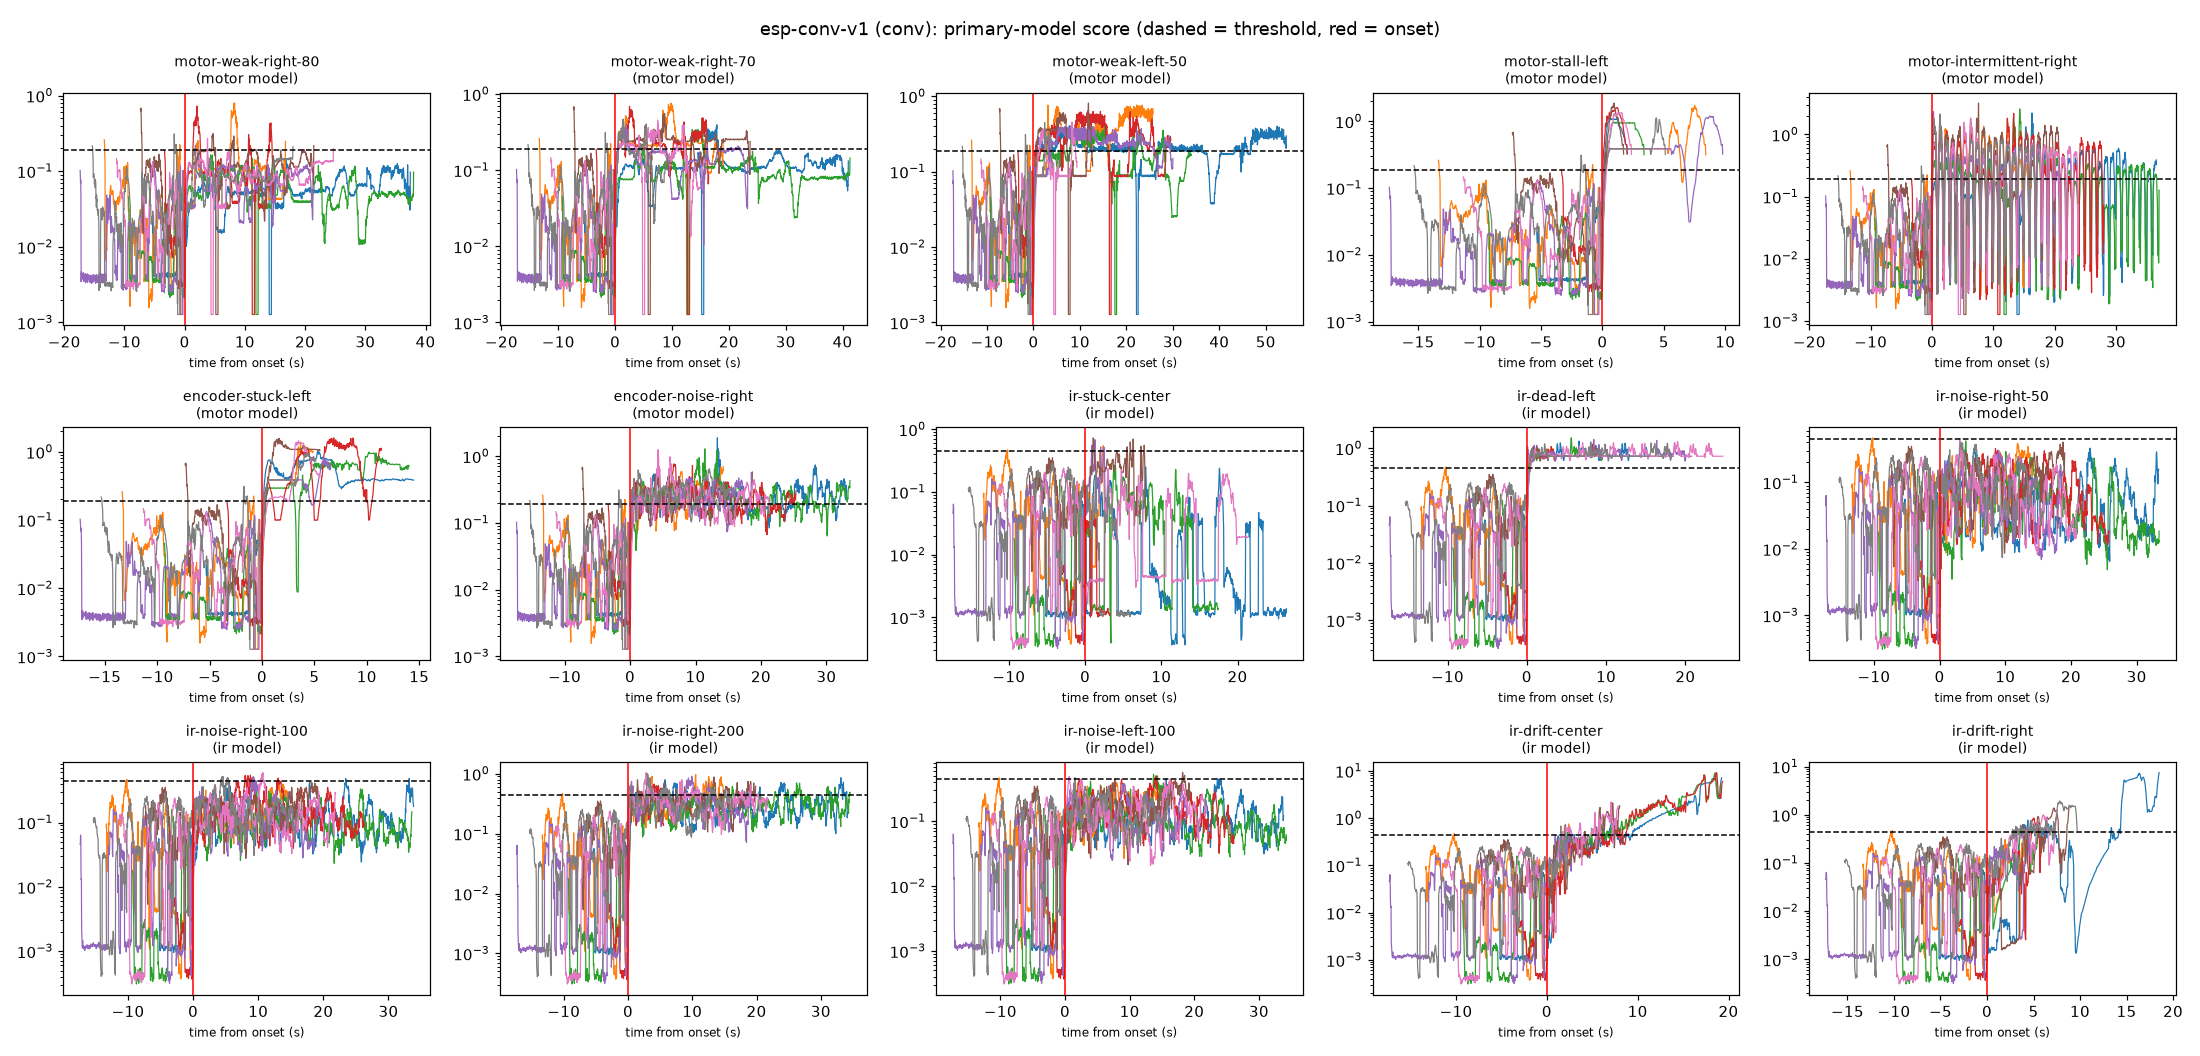
\includegraphics[width=\textwidth]{esp_fault_scores.png}
\caption{Score of each fault's own convolutional autoencoder on the 120 ESP
fault runs, aligned at the fault onset (red); dashed lines are thresholds.
Healthy segments stay below the threshold; most faults cross it within a second.
Light IR noise and IR drift remain close to the healthy range.}
\label{fig:faultscores}
\end{figure*}

\subsection{Detection limits}
In the earlier Supervisor-controlled study (64 healthy, 184 fault runs), a
severity sweep located the limits of the convolutional autoencoder
(Fig.~\ref{fig:sweep}): right-motor power loss of 20\% or more was detected in
7--8 of 8 runs, 15\% in 4/8 and 10\% or less essentially never; the
autoencoders outperformed a PCA baseline between 15\% and 30\% loss. IR noise
was detected reliably only at $\sigma=200$. An analysis of the 64 healthy runs
explains the IR limits: the ground sensors behave almost as on/off switches (fewer than 5\% of
readings between the dark and bright levels) and the centre sensor reads dark
97\% of the time, so moderate noise, slow drift or a sensor stuck at its
on-line value change little that a model can see.

\begin{figure}[t]
\centering
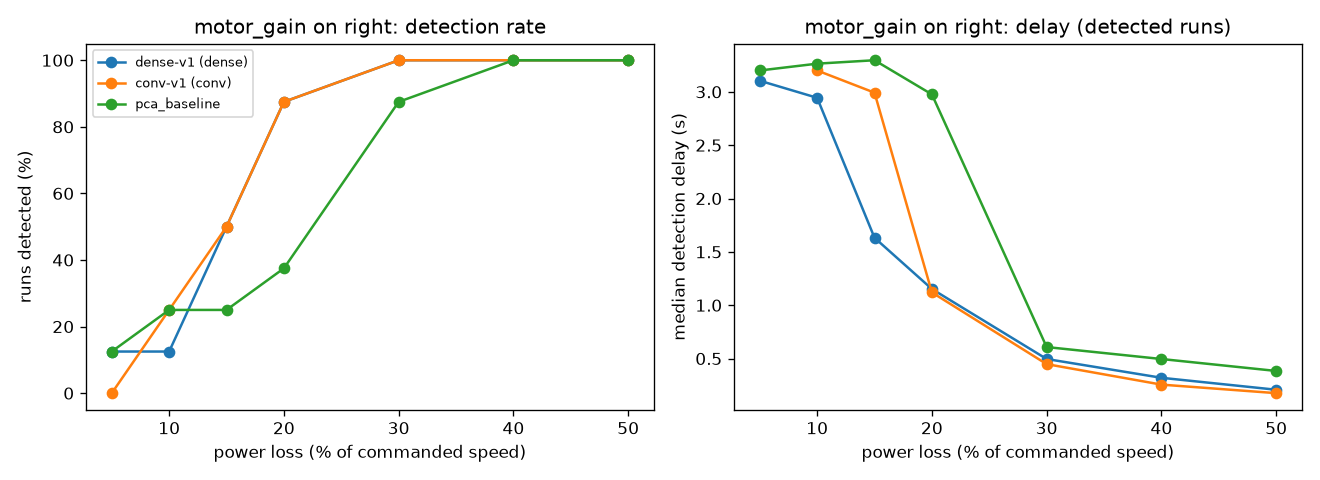
\includegraphics[width=\columnwidth]{severity_sweep_motor.png}
\caption{Severity sweep (Supervisor-controlled study): detection rate and median
delay against right-motor power loss for the dense and convolutional
autoencoders and a PCA baseline.}
\label{fig:sweep}
\end{figure}

\subsection{Navigation}
All routes A--D complete as round trips on the base track (including both
parallel edges) and on the two unseen tracks; the robot stops 0.1--2.0\,cm from
the destination node with a maximum path error of 2.5\,cm. On the unseen tracks,
8/8 healthy round trips completed on each, and all injected faults stopped the
robot and notified (track2 20/20, track3 16/16), with no model retraining.

\subsection{Computational cost}
Table~\ref{tab:latency} shows the per-frame cost on the ESP32-S3. Moving to
esp-dsp with weights in RAM cut the cost from 4.3\,ms for two models to 1.05\,ms
for three, and deploying the search winners to 0.81\,ms, about 2.5\% of the
32\,ms frame. About 51\,KB of weights reside in RAM; the firmware image is
0.94\,MB, leaving 70\% of the 3\,MB application partition free.

\begin{table}[t]
\caption{Detector time per 32\,ms frame on the ESP32-S3}
\label{tab:latency}
\centering
\footnotesize
\begin{tabular}{@{}lccc@{}}
\toprule
Detector & Scalar C, flash & esp-dsp, flash & esp-dsp, RAM \\
\midrule
Motor conv & 2.3\,ms & 1.96\,ms & 0.31\,ms \\
IR conv & 2.0\,ms & 1.51\,ms & 0.36\,ms \\
Motor GRU & -- & 1.32\,ms & 0.38\,ms \\
\midrule
\multicolumn{3}{@{}l}{All detectors, search winners deployed} & \textbf{0.81\,ms} \\
\bottomrule
\end{tabular}
\end{table}

\subsection{Quantization}
INT8 and INT16 versions built with ESP-DL~\cite{espdl} were 2.4--3.1$\times$
slower than float32 esp-dsp (737--821\,$\mu$s against 267--307\,$\mu$s) because
fixed per-layer overheads dominate models of 3k--17k multiply-accumulates. INT8
also broke the motor autoencoder: its healthy reconstruction error ($\approx$0.03)
is below INT8 rounding noise, causing 18/18 healthy validation alarms at the
float threshold. Float32 was kept.

\subsection{Hardware-aware architecture search}
The latencies of 967 architectures were measured on the ESP with a benchmark
firmware. A multi-objective TPE search~\cite{optuna} then maximized detections
on the tuning fault runs while minimizing the measured ESP time, and Pareto
candidates were retrained with the full budget and judged on held-out runs
(Table~\ref{tab:search}). For the motor detectors, smaller models were better on
every measure; the deployed system uses them. The smaller IR model detects more
held-out faults but adds two healthy test alarms, so it was not deployed.

\begin{table}[t]
\caption{Architecture search: deployed vs.\ best candidate (held-out runs)}
\label{tab:search}
\centering
\footnotesize
\setlength{\tabcolsep}{3.2pt}
\begin{tabular}{@{}llcccc@{}}
\toprule
Detector & Version & Detected & Delay & Healthy & ESP time \\
\midrule
\multirow{2}{*}{Motor conv} & original & 25/28 & 0.70\,s & 2/18 & 307\,$\mu$s \\
 & search & \textbf{28/28} & \textbf{0.40\,s} & 2/18 & \textbf{100\,$\mu$s} \\
\multirow{2}{*}{IR conv} & original & 17/32 & 2.75\,s & \textbf{0/18} & 294\,$\mu$s \\
 & search & \textbf{22/32} & 2.48\,s & 2/18 & \textbf{100\,$\mu$s} \\
\multirow{2}{*}{Motor GRU} & original & 27/28 & 0.16\,s & 0/18 & 267\,$\mu$s \\
 & search & \textbf{28/28} & \textbf{0.13\,s} & 0/18 & \textbf{127\,$\mu$s} \\
\bottomrule
\end{tabular}
\end{table}

\subsection{Live fault response}
In live runs with the deployed models, every healthy round trip finished without
an alarm frame; weak-motor faults (20\% and 30\% loss) ended in a fault stop in
8/8 runs with the first alarm 0.12--0.24\,s after onset (about 4\,s when the onset
fell inside a U-turn), and stuck-IR faults in 3/4 (the fourth began during a
U-turn and ended in a line-loss stop). Every stop produced exactly one
notification, and no alarm preceded any onset.

%=====================================================================
\section{Discussion and Limitations}
%=====================================================================
The motor and encoder faults are solved in this setting; the remaining gap is
in the IR channel. IR drift is detected in 4--6 of 8 runs and IR noise of
$\sigma\le100$ in 0--3 of 8 by the IR model, although the motor model reacts to
most noise runs because the line follower responds to the noisy signal. Per-sensor
maximum scoring, a sample-difference score and a one-step GRU forecaster did not
help: line crossings make healthy differences large and the forecaster copies a
slow ramp. A level check or a cross-sensor model that predicts each sensor from
the others and the motion are the next candidates; a thinner track line, which
would make the sensors graded rather than binary, would help both detection and
control. Other limits: faults that cause line loss during a U-turn are
unobservable (5 of 120 runs), each fault was injected at one onset time, and
results are from simulation, with a deterministic simulator that requires seeded
jitter for run diversity.

%=====================================================================
\section{Conclusion}
%=====================================================================
ESP-AGV shows that a low-cost microcontroller can drive an AGV and monitor it
with four learned and rule-based detectors in under 1\,ms per 32\,ms frame,
detecting every motor and encoder fault type within a fraction of a second, never
alarming before a fault and responding autonomously with a safe stop and a
notification. Measuring latency on the device was decisive: it showed that
float32 SIMD beats integer quantization at this model size and steered the
architecture search toward models that are both smaller and better.

%=====================================================================
\section*{GitHub Repository}
%=====================================================================
All code, models, manifests and evaluation reports are available at
\url{https://github.com/why-sobi/ESP-AGV}. The repository contains
\texttt{firmware/} (ESP-IDF firmware, generated model header, latency benchmark),
\texttt{simulation/} (Webots worlds and the bridge controller),
\texttt{maps/} (track images, graph maps, missions),
\texttt{scripts/} (map tools, telemetry collection, fault injection and
evaluation, training, export, replay and architecture search),
\texttt{models/}, \texttt{reports/}, \texttt{tests/}, and \texttt{docs/} with
usage instructions, design decisions and status. Every result in this paper is
reproducible from the committed configurations and manifests with the commands
in \texttt{docs/USAGE.md}.

%=====================================================================
\begin{thebibliography}{00}
\bibitem{esp32s3} Espressif Systems, ``ESP32-S3 Technical Reference Manual,'' 2023. [Online]. Available: \url{https://www.espressif.com}
\bibitem{webots} Cyberbotics Ltd., ``Webots: Open-source robot simulator.'' [Online]. Available: \url{https://cyberbotics.com}
\bibitem{espdsp} Espressif Systems, ``esp-dsp: DSP library for ESP-IDF.'' [Online]. Available: \url{https://github.com/espressif/esp-dsp}
\bibitem{gru} K. Cho \textit{et al.}, ``Learning phrase representations using RNN encoder--decoder for statistical machine translation,'' in \textit{Proc. EMNLP}, 2014, pp.~1724--1734.
\bibitem{sakurada2014} M. Sakurada and T. Yairi, ``Anomaly detection using autoencoders with nonlinear dimensionality reduction,'' in \textit{Proc. MLSDA Workshop}, 2014, pp.~4--11.
\bibitem{optuna} T. Akiba, S. Sano, T. Yanase, T. Ohta, and M. Koyama, ``Optuna: A next-generation hyperparameter optimization framework,'' in \textit{Proc. ACM SIGKDD}, 2019, pp.~2623--2631.
\bibitem{espdl} Espressif Systems, ``ESP-DL: Deep-learning library for Espressif SoCs.'' [Online]. Available: \url{https://github.com/espressif/esp-dl}
\end{thebibliography}

\end{document}
